\documentclass[tikz,border=4pt]{standalone}
\usepackage{pgfplots}
\pgfplotsset{compat=1.18}
\usepgfplotslibrary{fillbetween}
\usetikzlibrary{arrows.meta,positioning,calc,shapes.geometric}
\begin{document}
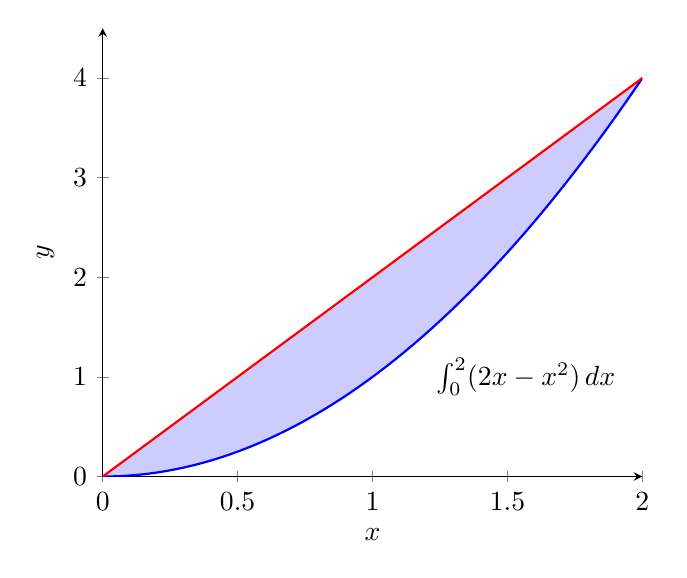
\begin{tikzpicture}
  \begin{axis}[axis lines=left, xlabel=$x$, ylabel=$y$, domain=0:2, samples=60, enlargelimits=false, ymax=4.5]
    \addplot[name path=f, thick, blue] {x^2};
    \addplot[name path=g, thick, red] {2*x};
    \addplot[blue!20] fill between[of=f and g];
    \node[anchor=west] at (axis cs:1.2,1) {$\int_0^2 (2x-x^2)\,dx$};
  \end{axis}
\end{tikzpicture}
\end{document}
